%---------------------------------
\chapter{Birkhoff--von~Neumannの定理}
\label{chap:vonNeumann}
%---------------------------------
サイズ$N$の正方行列$\bm{D}$が二重確率行列であるとき,$\bm{D}$はサイズ$N$の全てのパーミュテーション行列$\{\bm{P}_i\}_{i=1}^{N!}$の凸結合で表せる.
即ち,凸結合の係数$\sigma_i \geq 0$を用いて次式が成立する.
\begin{align}
    \bm{D} = \sum_{i=1}^{N!} \sigma_i \bm{P}_i
\end{align}
但し,$\sigma_i$は凸結合係数であるため,$\sum_{i=1}^{N!} \sigma_i = 1$を満たす.
%---------------------------------
\chapter{人工データに対する予測結果}
\label{chap:artificial}
%---------------------------------

\ref{chap:ex}章で掲載した人工データに対する実験結果の他にも,4行,8行毎に各周波数成分をシャッフルした場合の実験も行った.
以下に実験結果を掲載する.

%%%%%%%%%%%%%%%%%%%%%%%%%%%%
\begin{figure*}[!t]
    \centering
    \subfloat[Accuracy for training and validation data.]{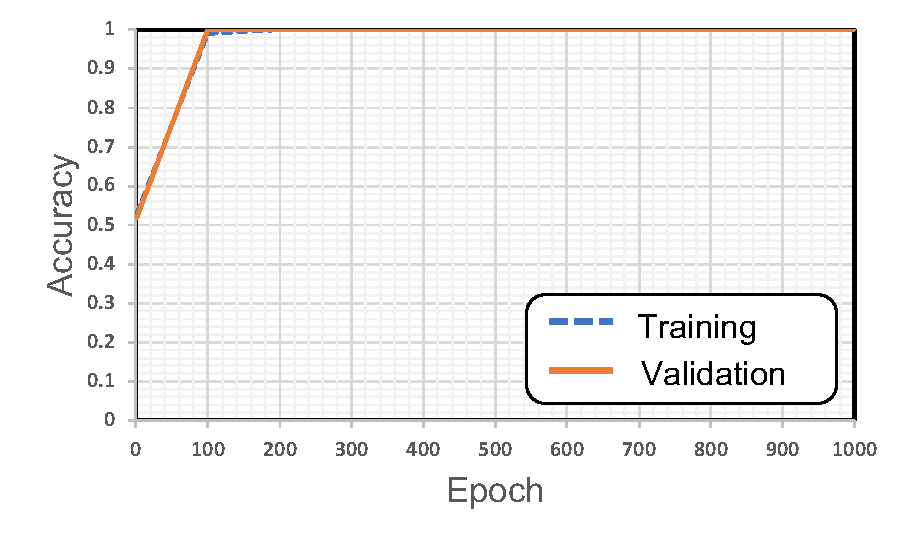
\includegraphics[clip, width=4.5in]{figures/graph/01mat_4block.pdf}
    \vspace{-15pt}
    \label{fig:acc_01mat_4block}}
    \\
    \subfloat[Input matrices with permutation problem (upper) and permutation-aligned matrices using predicted results (bottom).]{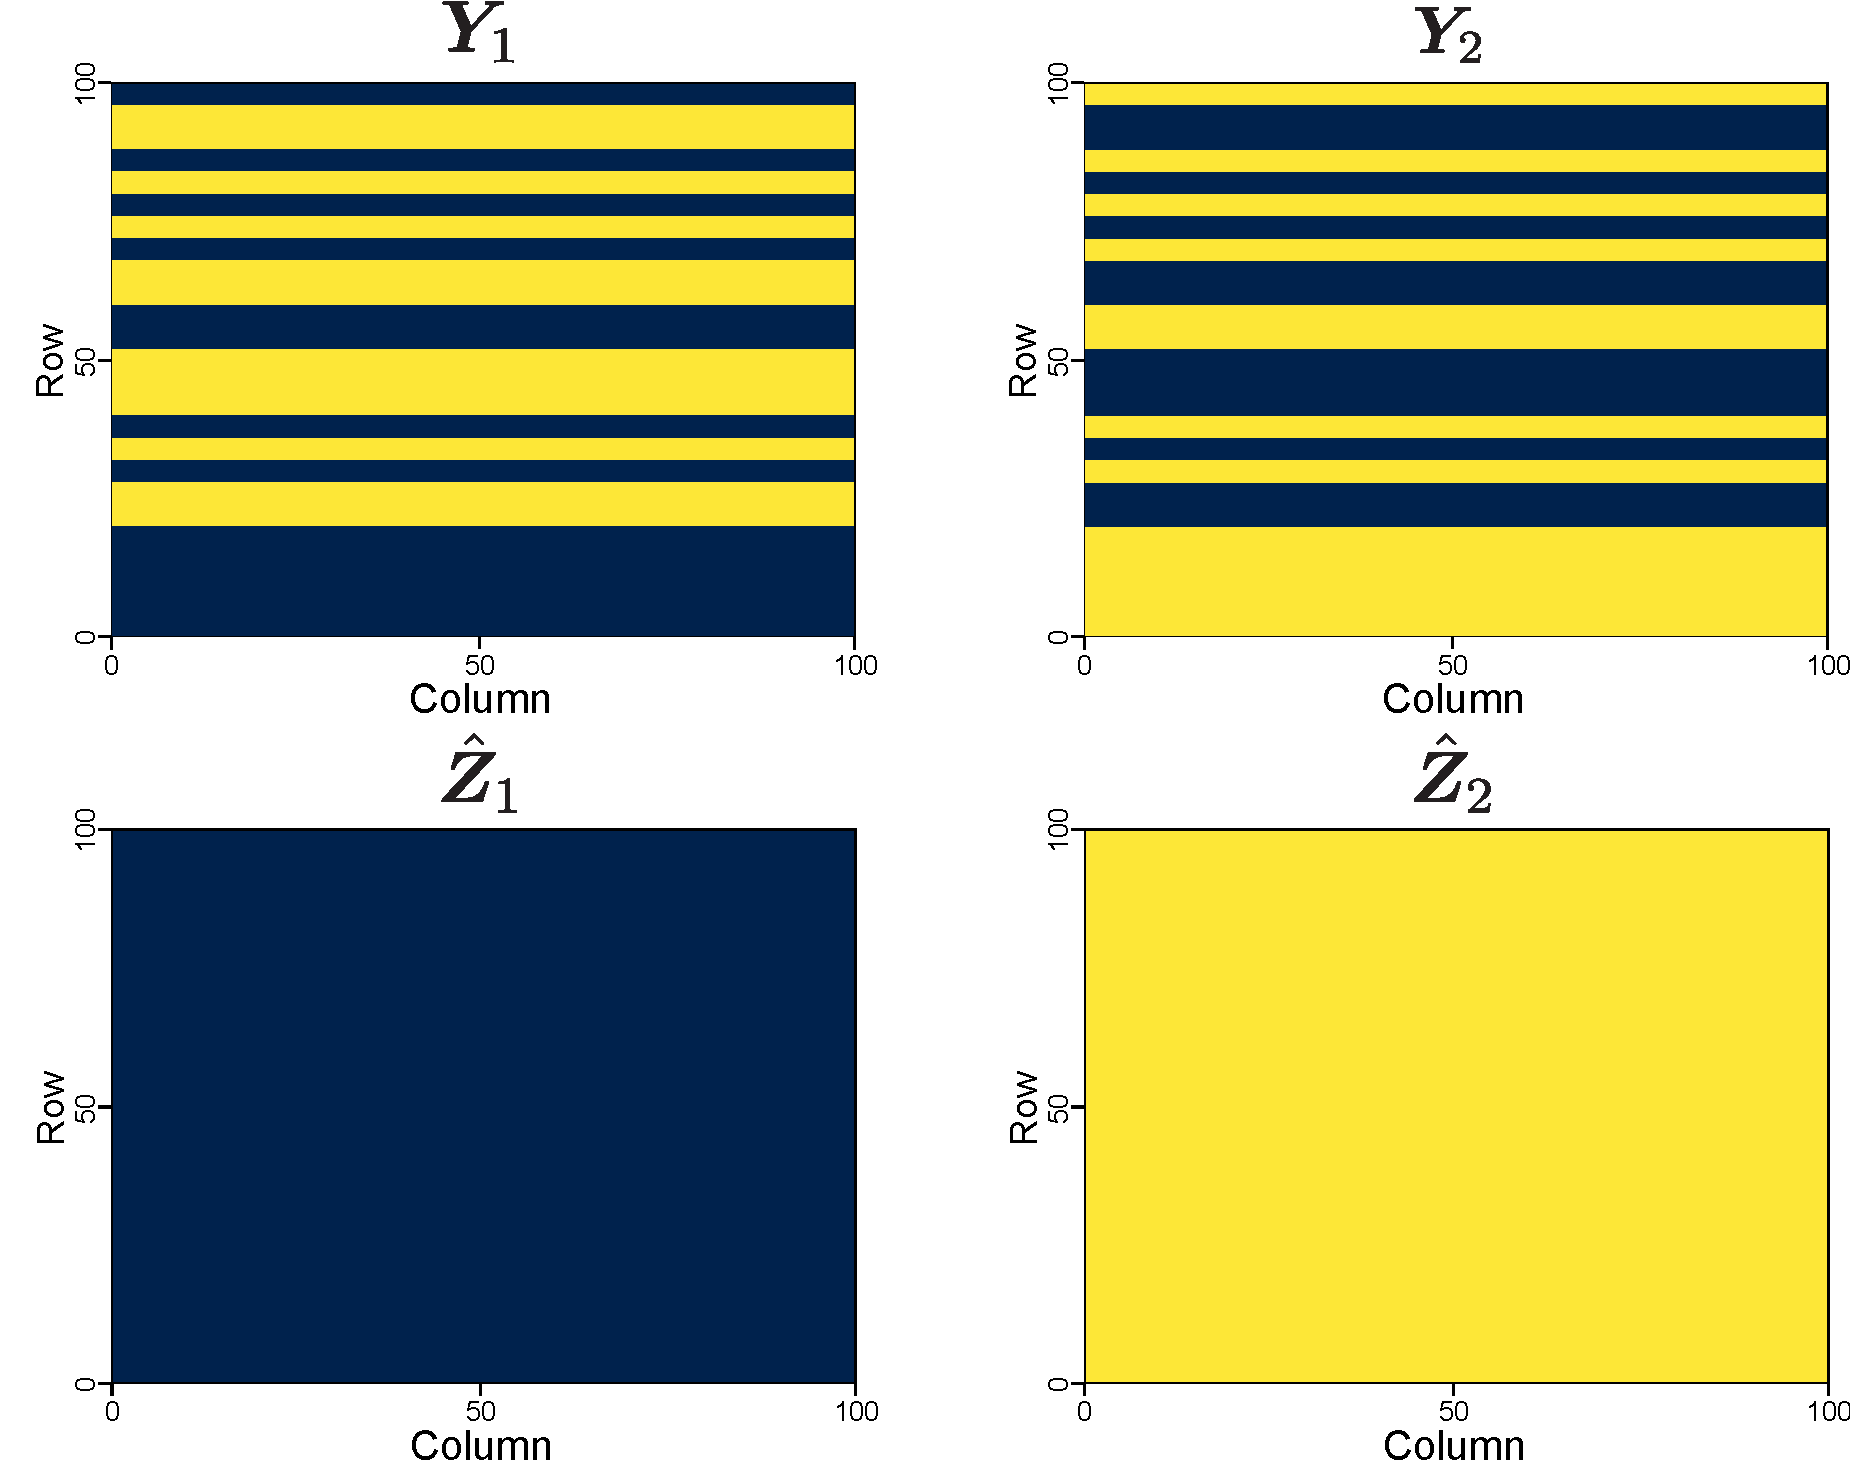
\includegraphics[clip, width=5.0in]{figures/01mat_4block.pdf}
    \label{fig:spec_01mat_4block}}  
    \caption{Experimental results with $\gamma=4$ using artificial source matrices of Fig.~\ref{fig:01mat_spec}.}
    \label{fig:01mat_4block}
\end{figure*}
%%%%%%%%%%%%%%%%%%%%%%%%%%%%

%%%%%%%%%%%%%%%%%%%%%%%%%%%%
\begin{figure*}[!t]
    \centering
    \subfloat[Accuracy for training and validation data.]{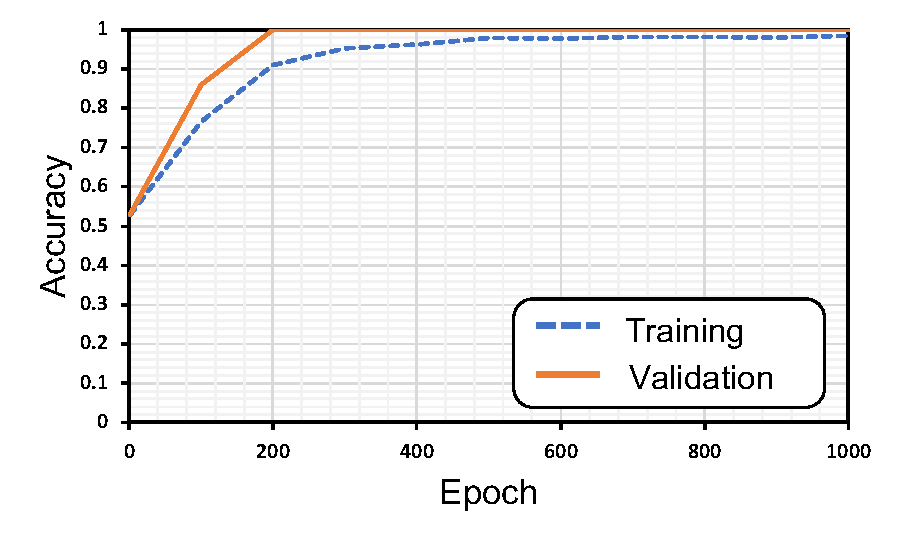
\includegraphics[clip, width=4.5in]{figures/graph/25stripe_4block.pdf}
    \vspace{-15pt}
    \label{fig:acc_25mat_4block}}
    \\
    \subfloat[Input matrices with permutation problem (upper) and permutation-aligned matrices using predicted results (bottom).]{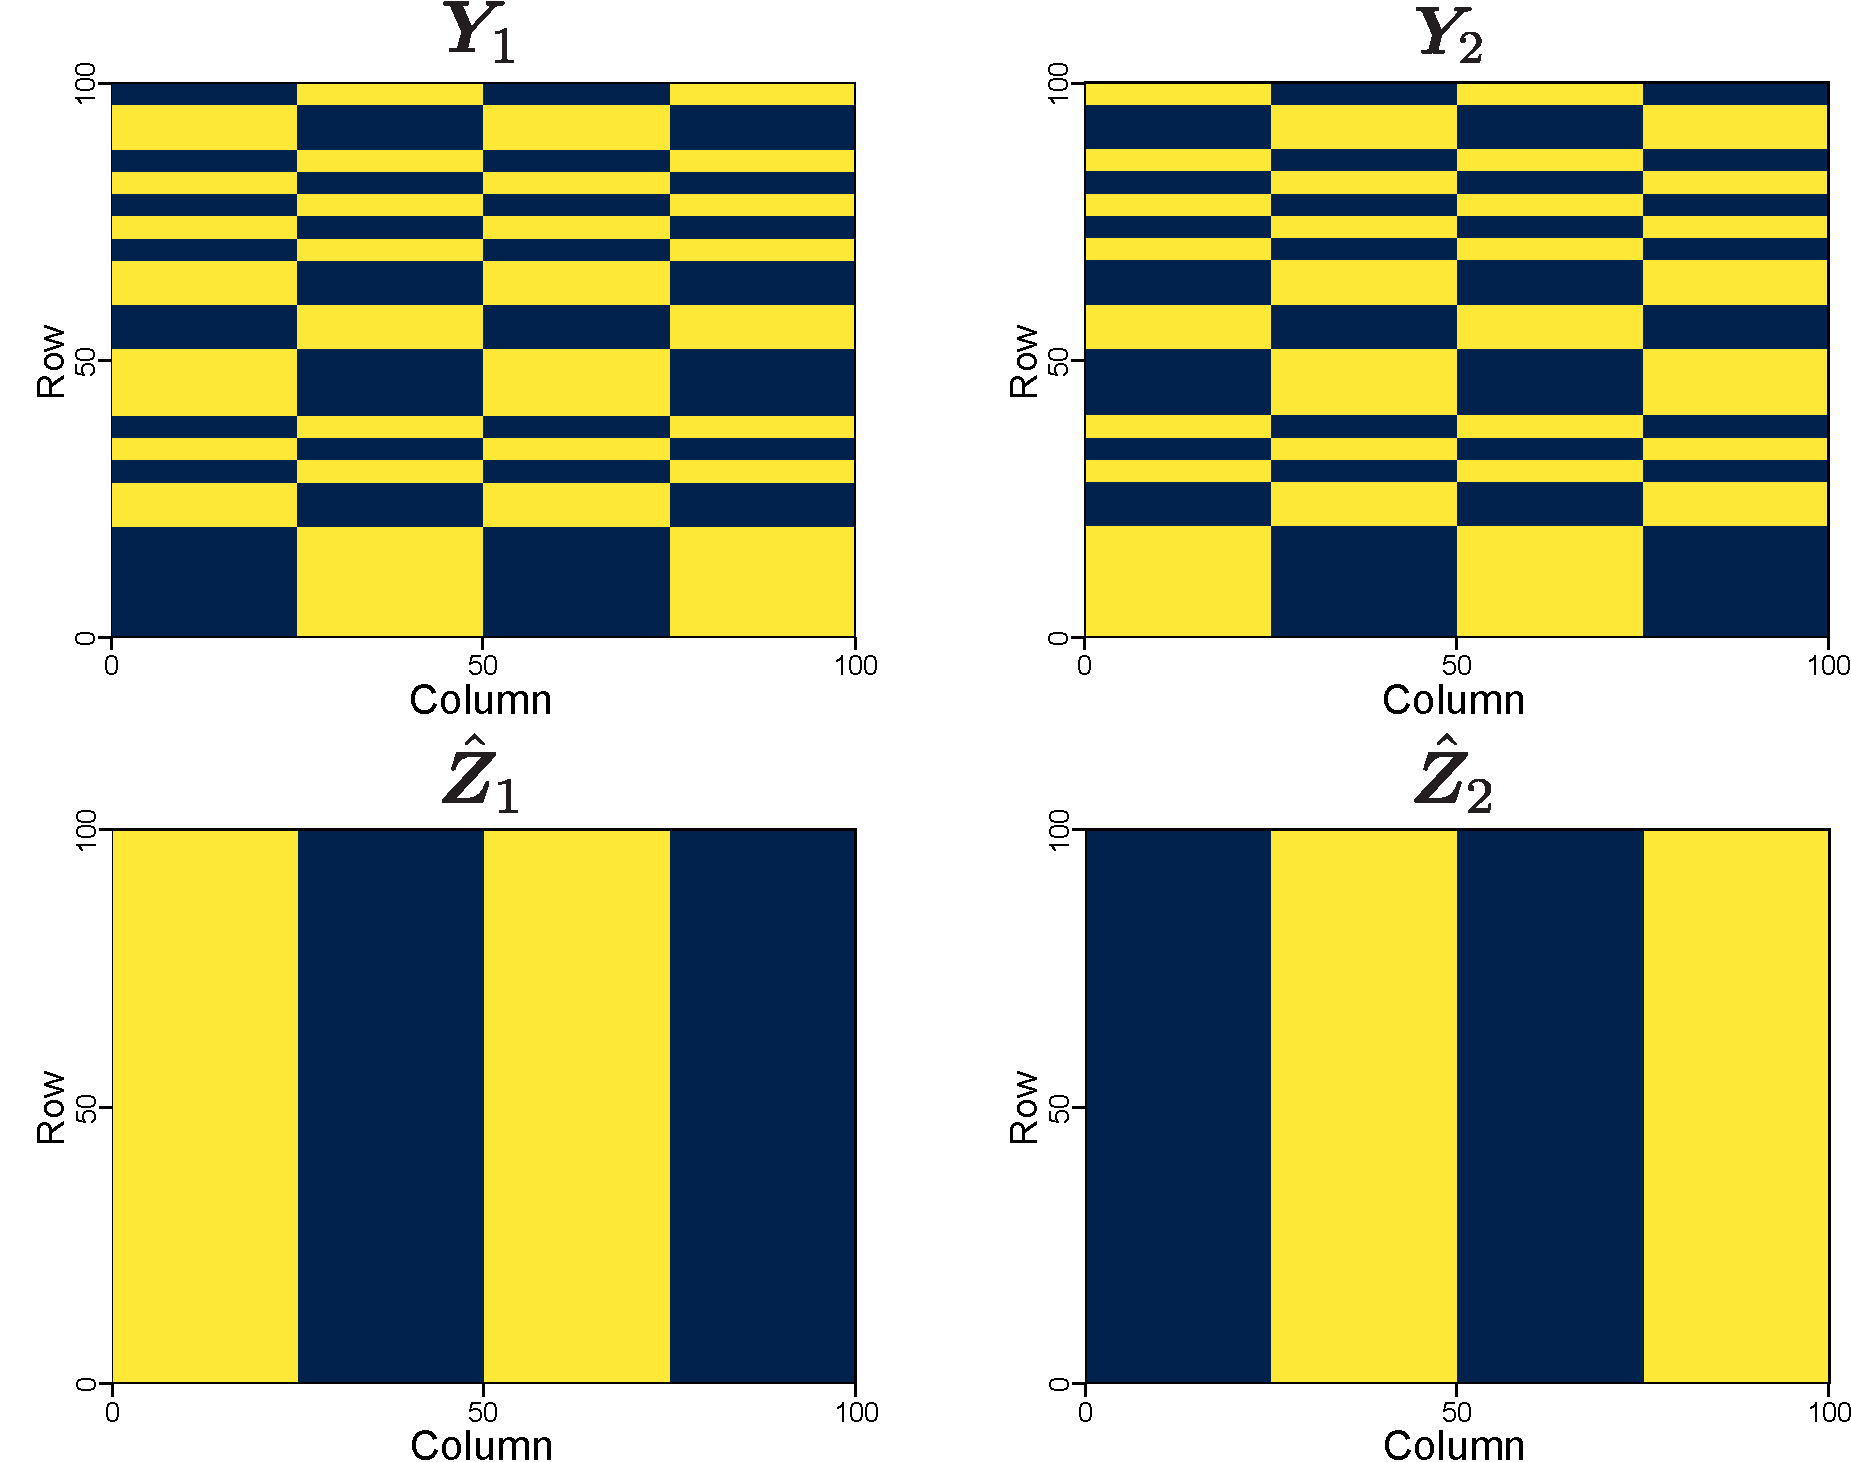
\includegraphics[clip, width=5.0in]{figures/25stripe_4block.pdf}
    \label{fig:spec_25mat_4block}}  
    \caption{Experimental results with $\gamma=4$ using artificial source matrices of Fig.~\ref{fig:25stripe_spec}.}
    \label{fig:25mat_4block}
\end{figure*}
%%%%%%%%%%%%%%%%%%%%%%%%%%%%

%%%%%%%%%%%%%%%%%%%%%%%%%%%%
\begin{figure*}[!t]
    \centering
    \subfloat[Accuracy for training and validation data.]{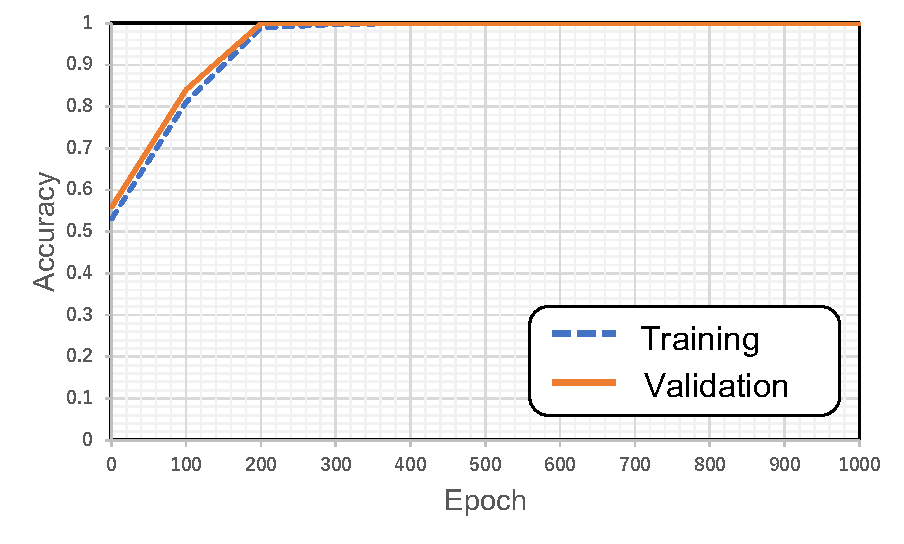
\includegraphics[clip, width=4.5in]{figures/graph/stripe_4block.pdf}
    \vspace{-15pt}
    \label{fig:acc_stripe_4block}}
    \\
    \subfloat[Input matrices with permutation problem (upper) and permutation-aligned matrices using predicted results (bottom).]{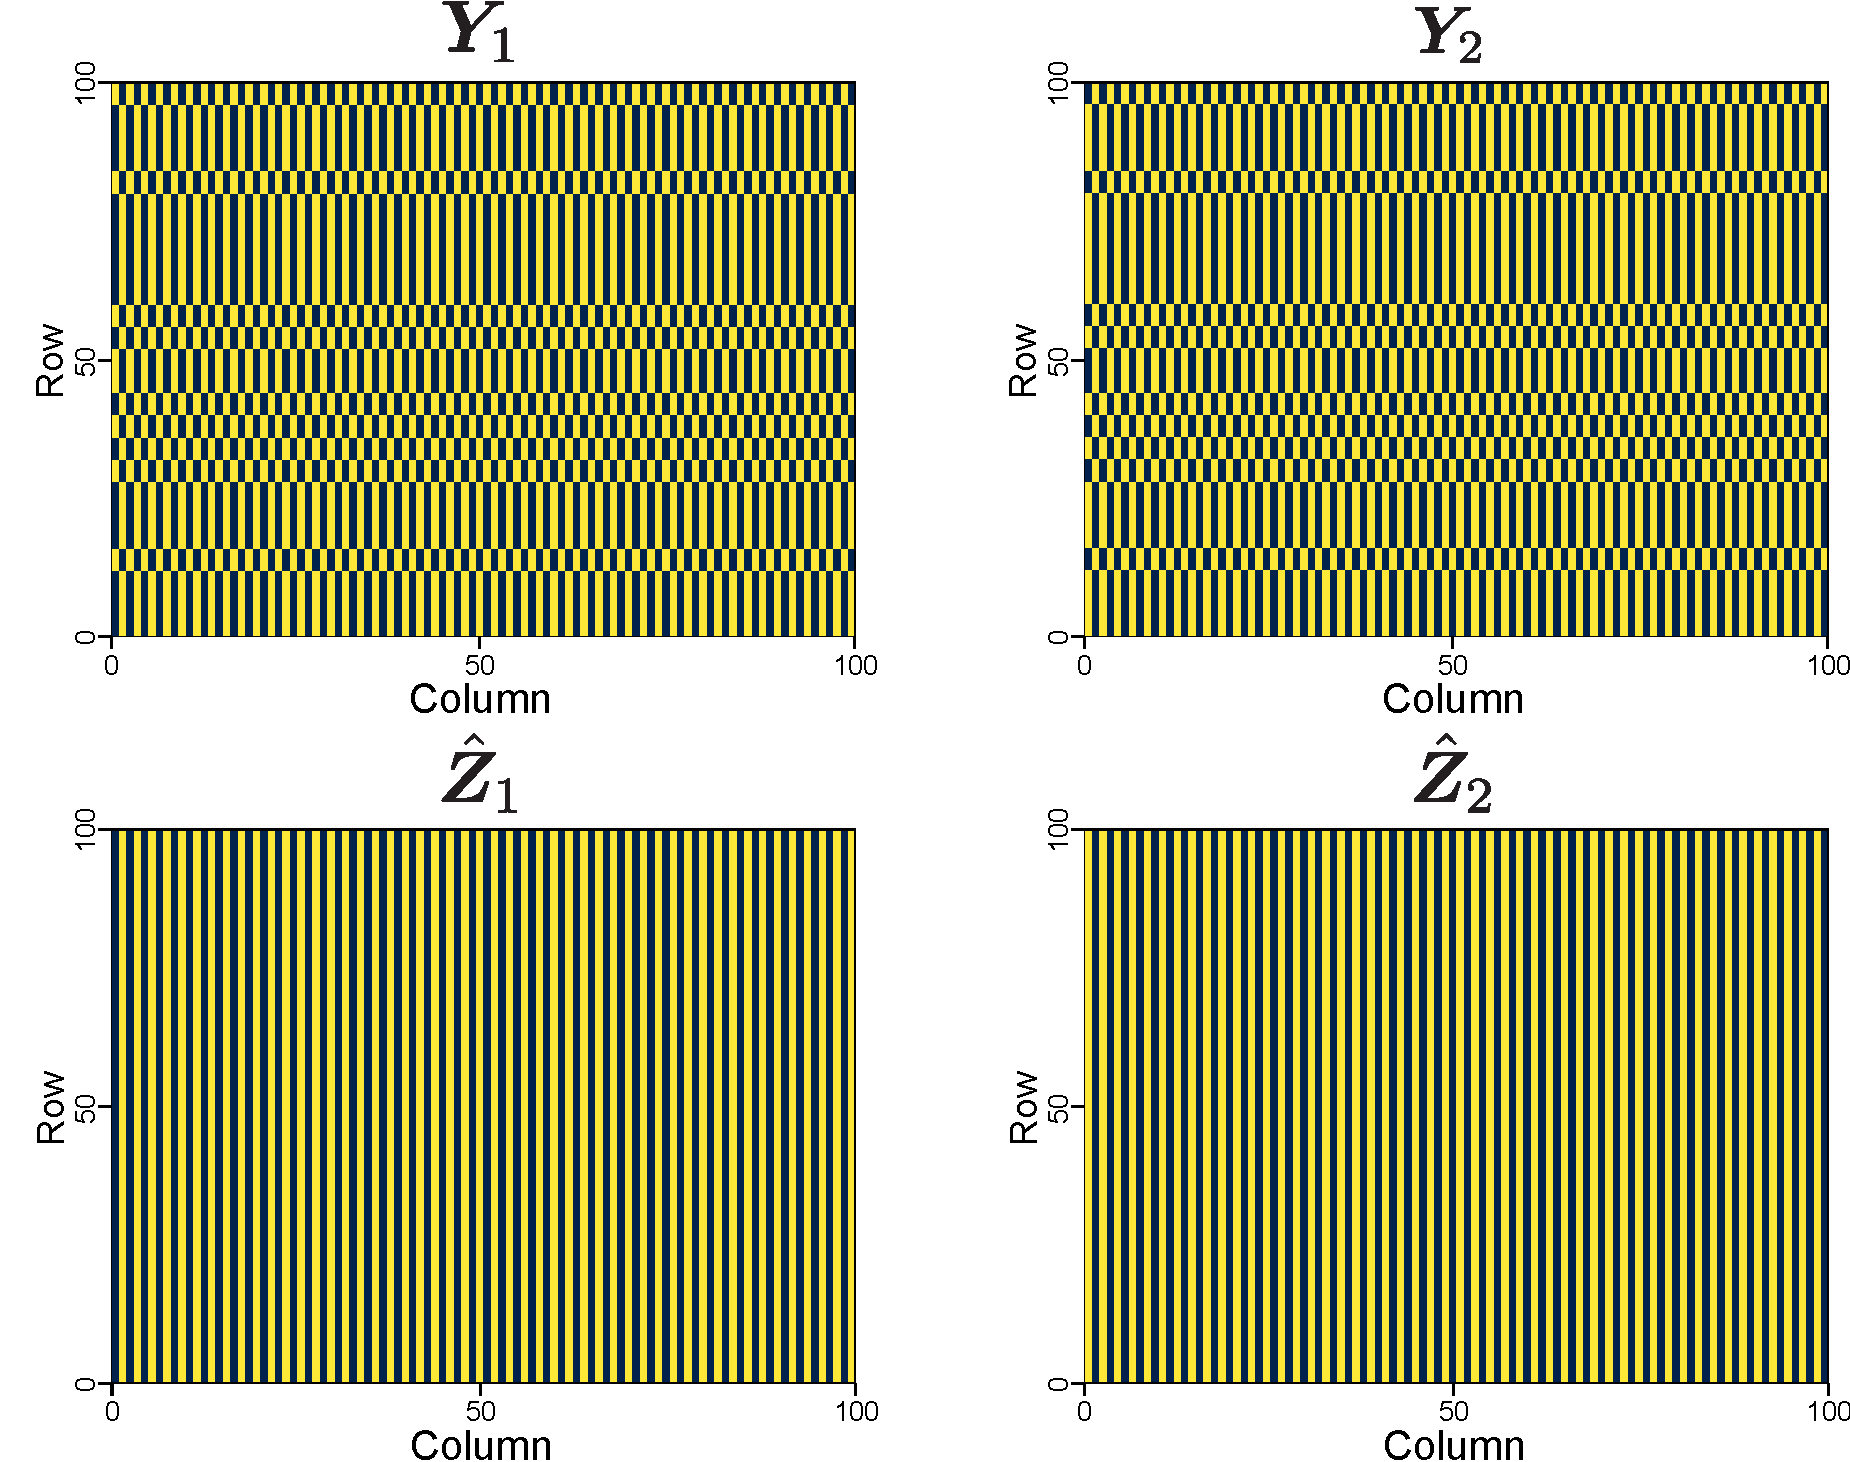
\includegraphics[clip, width=5.0in]{figures/stripe_4block.pdf}
    \label{fig:spec_stripe_4block}}  
    \caption{Experimental results with $\gamma=4$ using artificial source matrices of Fig.~\ref{fig:stripe_spec}.}
    \label{fig:stripe_4block}
\end{figure*}
%%%%%%%%%%%%%%%%%%%%%%%%%%%%

%%%%%%%%%%%%%%%%%%%%%%%%%%%%
\begin{figure*}[!t]
    \centering
    \subfloat[Accuracy for training and validation data.]{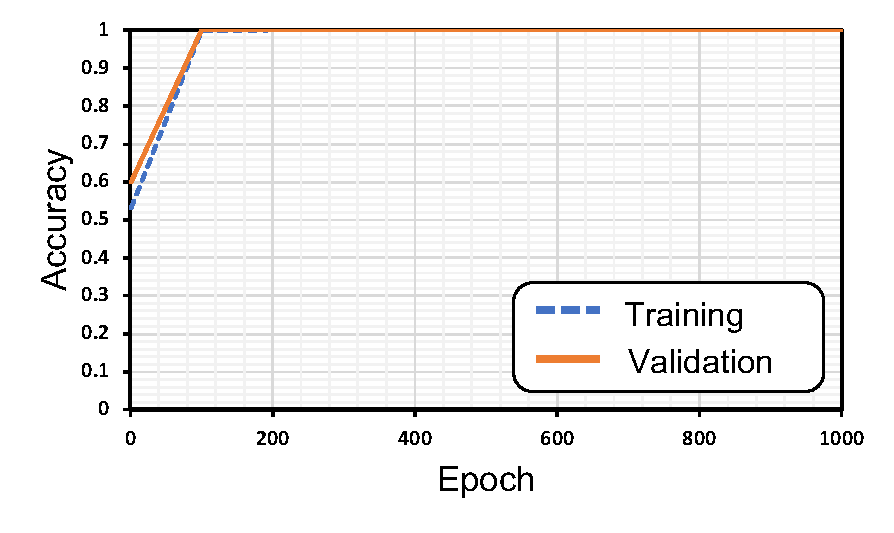
\includegraphics[clip, width=4.5in]{figures/graph/01mat_8block.pdf}
    \vspace{-15pt}
    \label{fig:acc_01mat_8block}}
    \\
    \subfloat[Input matrices with permutation problem (upper) and permutation-aligned matrices using predicted results (bottom).]{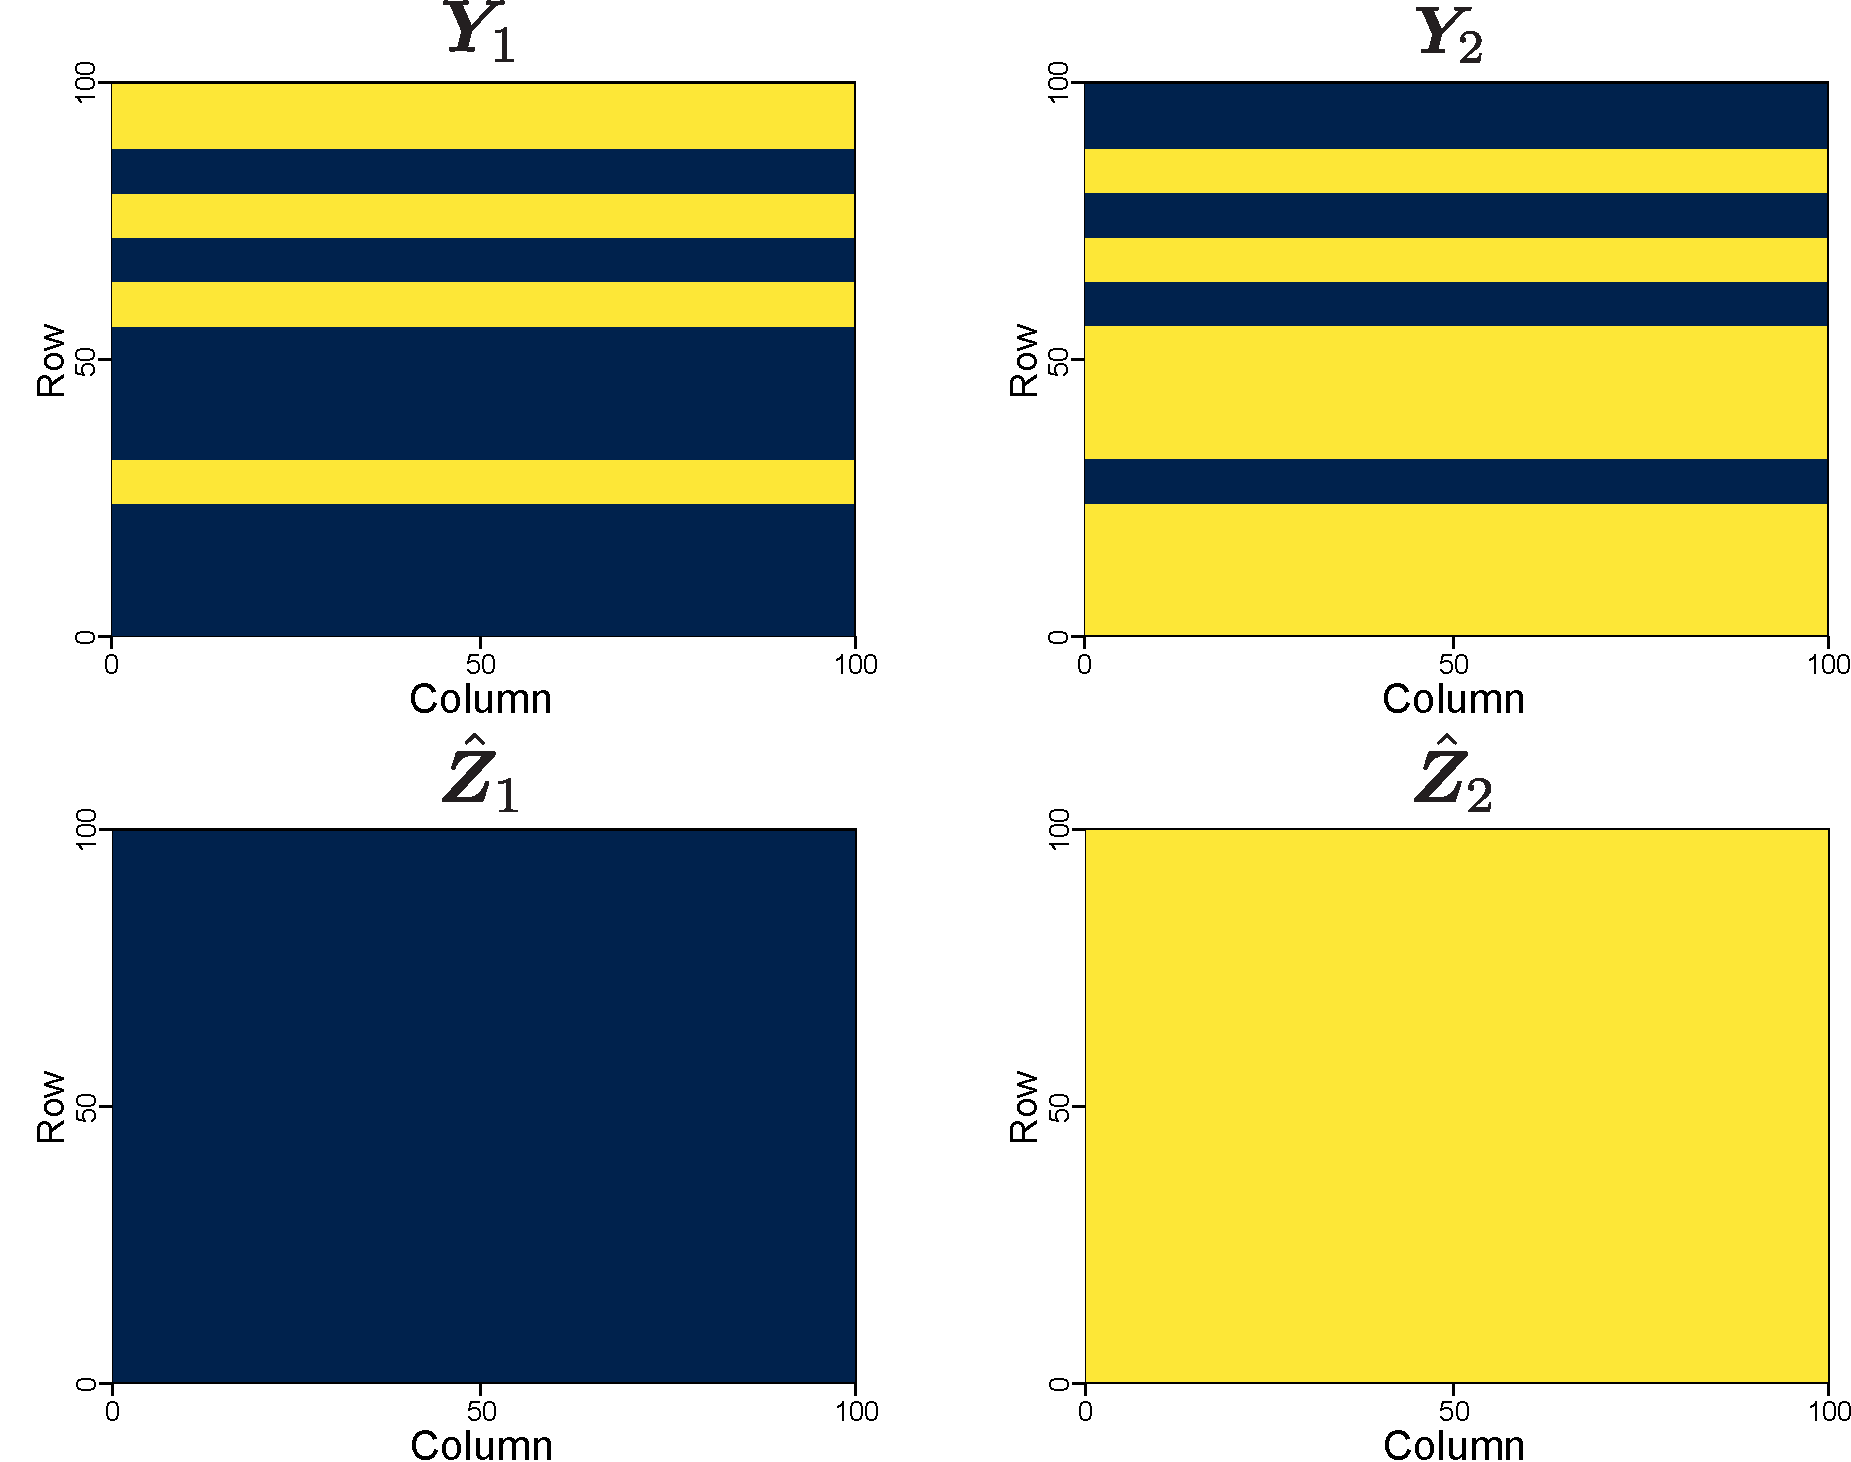
\includegraphics[clip, width=5.0in]{figures/01mat_8block.pdf}
    \label{fig:spec_01mat_8block}}  
    \caption{Experimental results with $\gamma=8$ using artificial source matrices of Fig.~\ref{fig:01mat_spec}.}
    \label{fig:01mat_8block}
\end{figure*}
%%%%%%%%%%%%%%%%%%%%%%%%%%%%

%%%%%%%%%%%%%%%%%%%%%%%%%%%%
\begin{figure*}[!t]
    \centering
    \subfloat[Accuracy for training and validation data.]{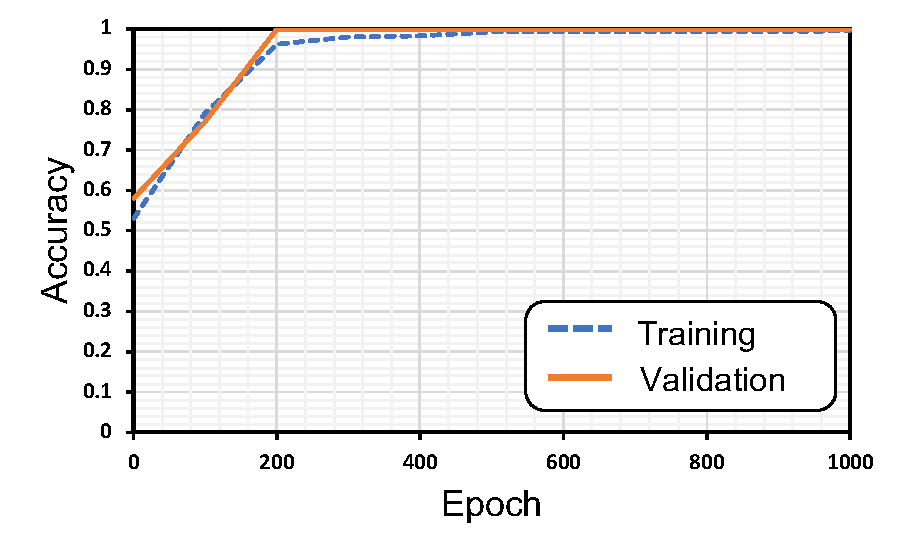
\includegraphics[clip, width=4.5in]{figures/graph/25stripe_8block.pdf}
    \vspace{-15pt}
    \label{fig:acc_25mat_8block}}
    \\
    \subfloat[Input matrices with permutation problem (upper) and permutation-aligned matrices using predicted results (bottom).]{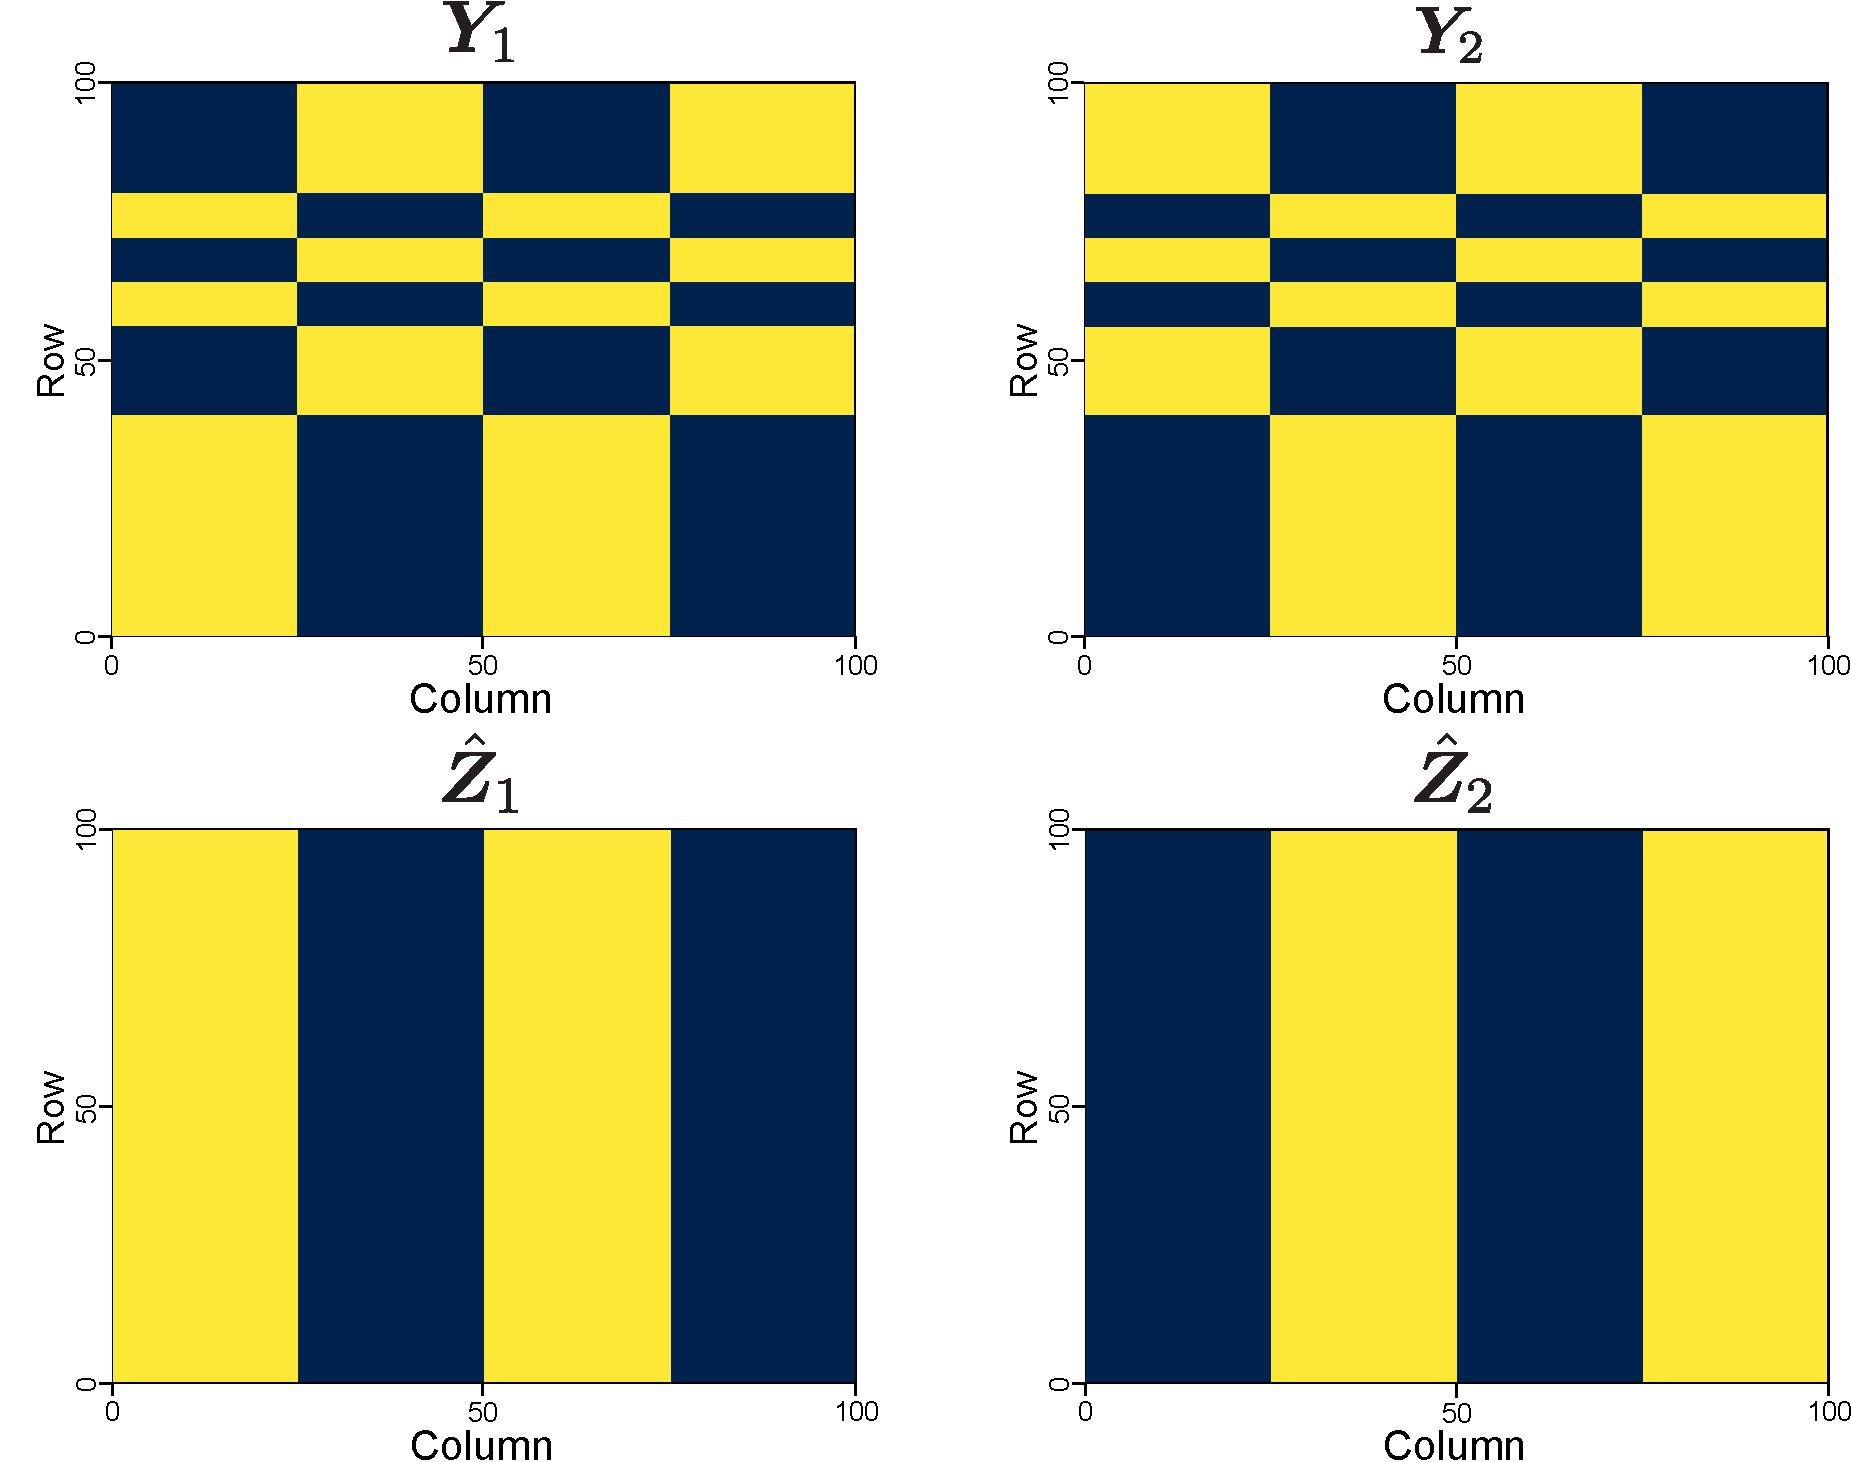
\includegraphics[clip, width=5.0in]{figures/25stripe_8block.pdf}
    \label{fig:spec_25mat_8block}}  
    \caption{Experimental results with $\gamma=8$ using artificial source matrices of Fig.~\ref{fig:25stripe_spec}.}
    \label{fig:25mat_8block}
\end{figure*}
%%%%%%%%%%%%%%%%%%%%%%%%%%%%

%%%%%%%%%%%%%%%%%%%%%%%%%%%%
\begin{figure*}[!t]
    \centering
    \subfloat[Accuracy for training and validation data.]{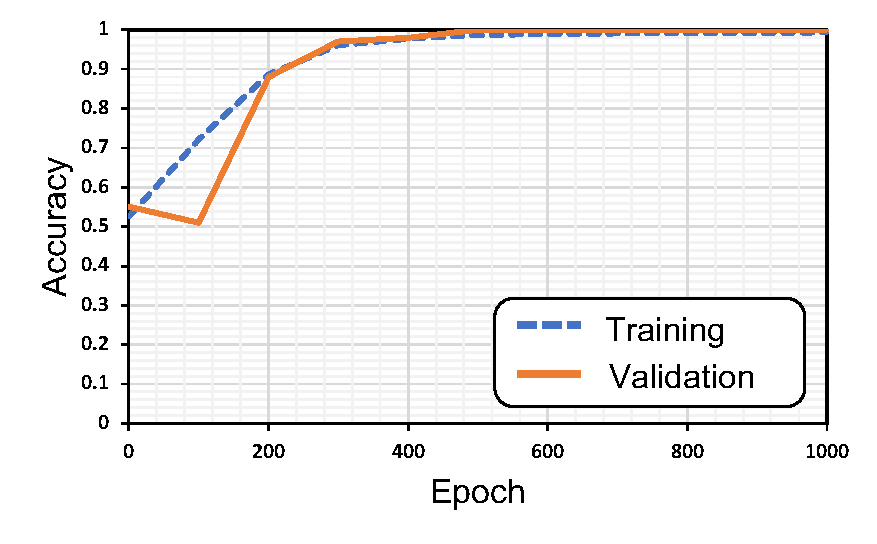
\includegraphics[clip, width=4.5in]{figures/graph/stripe_8block.pdf}
    \vspace{-15pt}
    \label{fig:acc_stripe_8block}}
    \\
    \subfloat[Input matrices with permutation problem (upper) and permutation-aligned matrices using predicted results (bottom).]{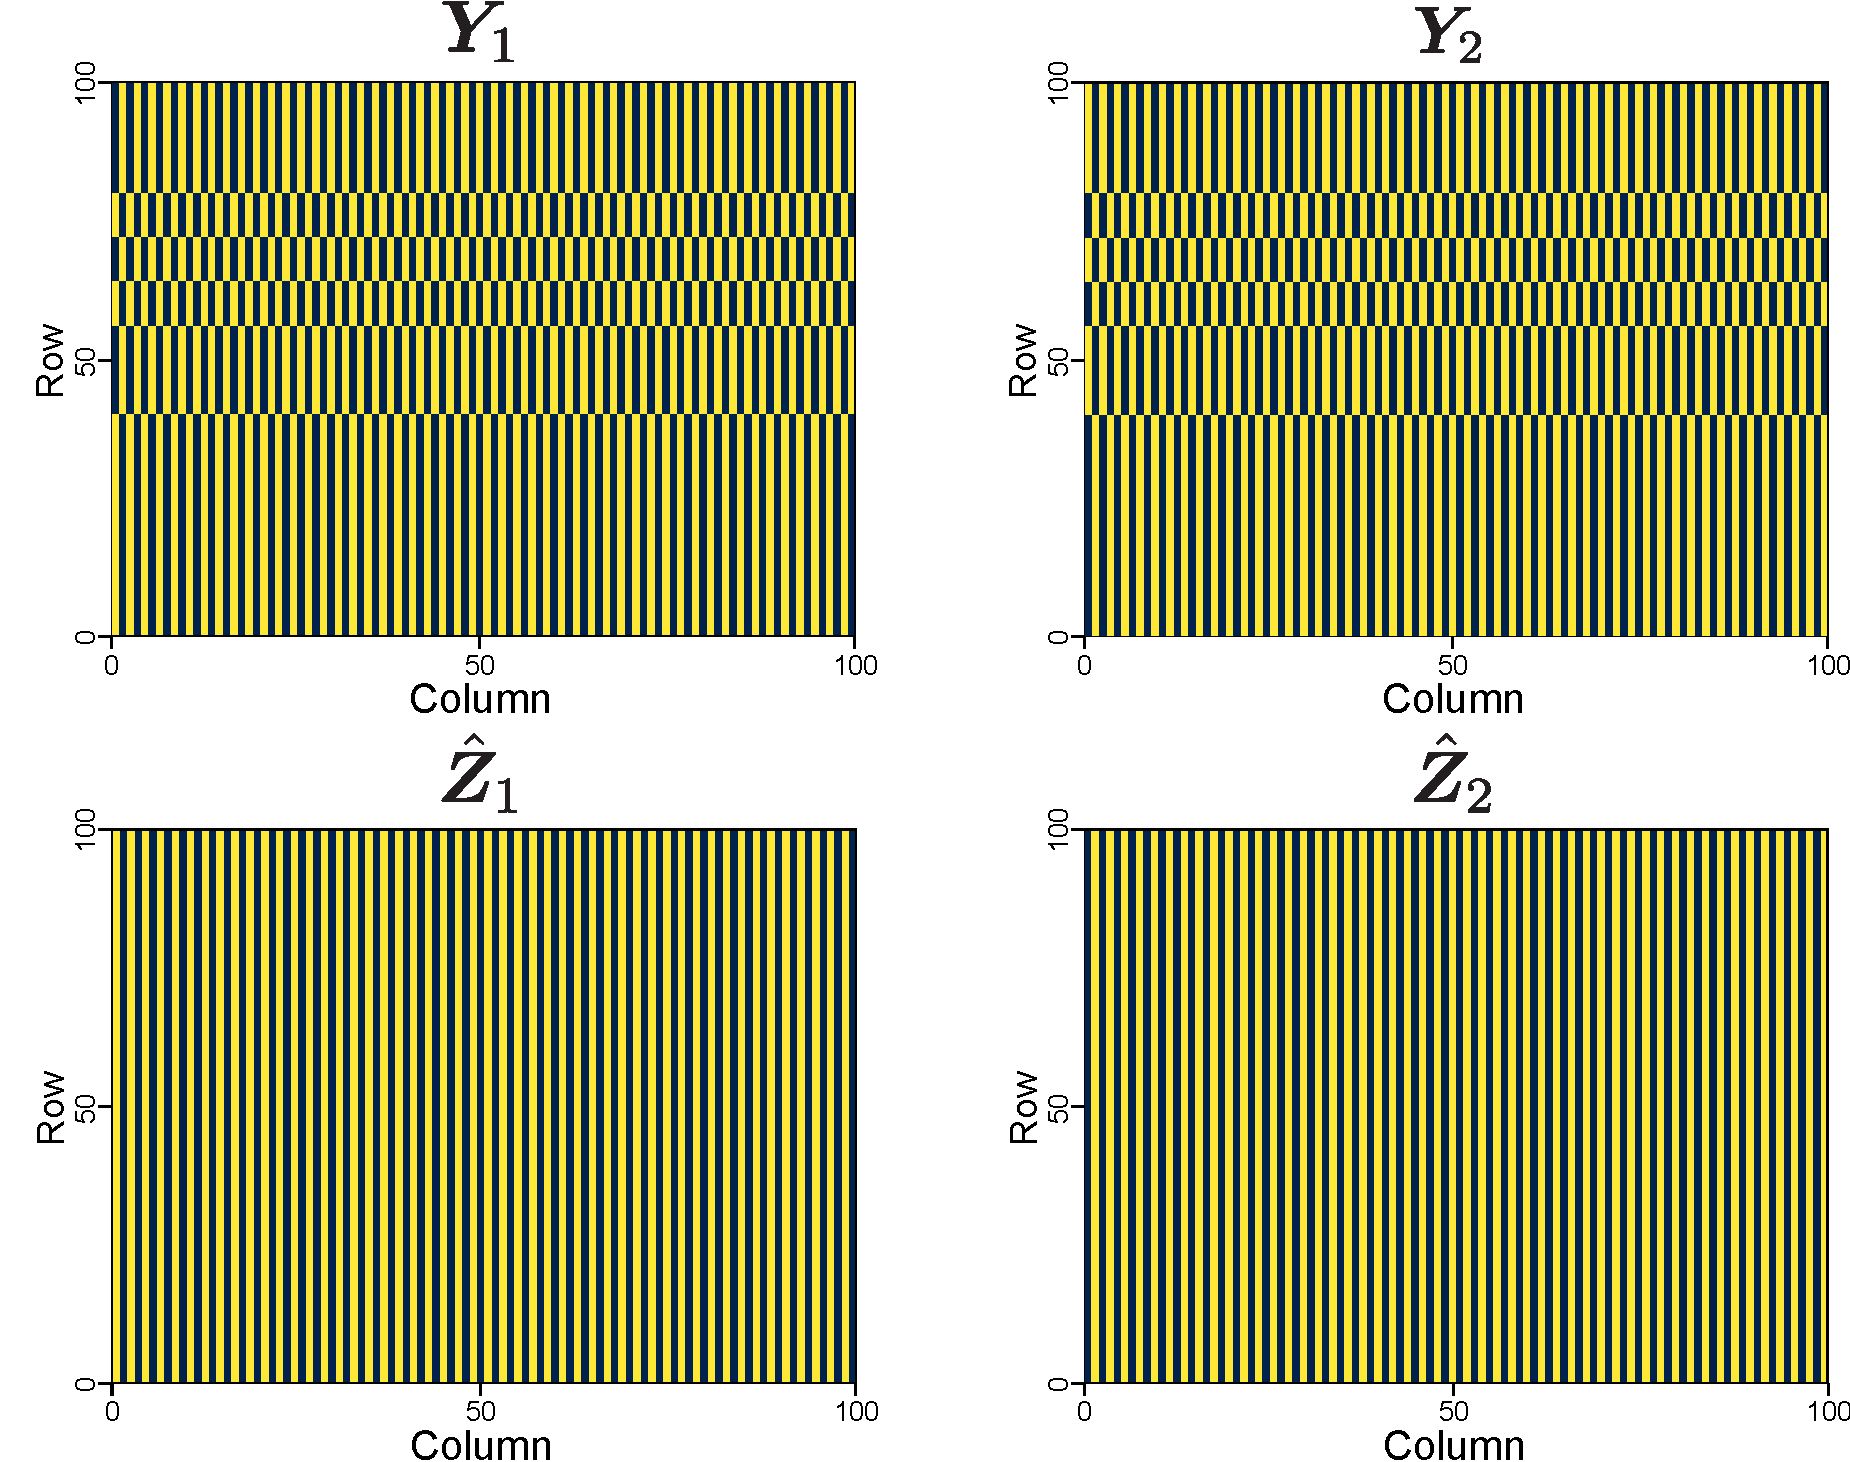
\includegraphics[clip, width=5.0in]{figures/stripe_8block.pdf}
    \label{fig:spec_stripe_8block}}  
    \caption{Experimental results with $\gamma=8$ using artificial source matrices of Fig.~\ref{fig:stripe_spec}.}
    \label{fig:stripe_8block}
\end{figure*}
%%%%%%%%%%%%%%%%%%%%%%%%%%%%
